\documentclass{article}
\usepackage{gensymb}
\usepackage{graphicx}
\graphicspath{ {./res-images/} }
\usepackage{listings}
\begin{document}

\title{Building Resilience Vaccine Distribution}
\author{Saransh Sharma }
\date{January 2021}


\maketitle


\abstract

The COVID-19 pandemic has been one of the most influential pandemics in a century. Conventional life has been disrupted on a global scale, with rampant disease transmission leading to an unusual number of deaths. To take measures for this widespread virus transmission, vaccines have been developed since the early emergence of the pandemic. However, due to the substantial burden on the medical community and the gradual collapse of economies worldwide, vaccine testing processes were expedited to stabilize the uncontrolled virus. The development of some vaccines was accelerated by combining multiple phases of vaccine testing by running them in parallel. Once developed, the vaccines received early or limited approval. Yet, the distribution infrastructure and strategies remain undetermined, especially in necessary regions. It has impacted the timely delivery of vaccines to needy people and management to control the pandemic at an expected level. This study aims to address some of the deficiencies in the administration and distribution infrastructure of vaccines while proposing efficient and systematized strategies.

\section{Introduction}
Andrew Heinrich from Yale University also stated that the COVID-19 vaccination campaign is the most rapid and the largest vaccination drive in human history that created a supply chain and distribution challenges. From manufacturing to the transportation to storage and vaccination, each layer of the event has myriad complexities and challenges to deal with. It made us incapable of vaccinating all people at once and forced to make strategic and equitable planning and decisions about vaccination drives worldwide.  

The COVID-19 vaccines, Covaxin and AstraZeneca Oxford jab, in India, are approved for restricted use in an emergency situation in the public interest as an abundant precaution, in clinical trial mode, especially in the context of infection by mutant strains.\footnote{https://www.bbc.com/news/world-asia-india-55534902}, though there are serious concerns on lack of evidence and unsatisfactory scientific evidence of safety and efficacy for the vaccines produced in India.\footnote{bae 2020 challenges} 

India planned to vaccinate about 300 million people from January to July 2021, first vaccinating people above age 50. India is the second most populated nation, and most of the population is in rural and remote areas. Three things should have been ensured to be in place before starting the vaccination drive, that are:

\begin{itemize}
\item Developing national vaccination plan 
\item Vaccine supplies (cold storage, syringes, distribution, needles), regulatory vaccine approval
\item Vaccine safety systems
\item Staff implementing the drive (vaccinators, documentors) and their training
\Strengthening data collection, tracking, reporting, and analysing systems
\item Plan public health campaigns to build trust and generate COVID-19 vaccine demand
\item People to be vaccinated
\end{itemize}

The vaccination drive needs a strong vaccine intelligence network to ensure the last-mile delivery of the vaccine. Before that, there needs to be a dedicated focus on filling the gaps in the distribution network and resources. Presently, the world’s manufacturing processes, as well as supply chains, are significantly underprepared for the task of widespread vaccine distribution in a targeted short period of span [3]. Each country has its own logistical and ethical challenges, but low and middle income countries face particular challenges due to insufficient resources and support systems.  

COVID-19 vaccine movement in India possesses unknown and unresolved issues that have caused delays in the vaccination. Inefficiency in the supply chain and the lack of adequate infrastructure are primarily impacted the on-time delivery of vaccines at different locations. One of the major challenges in the process is an inadequate cold chain and distribution infrastructure. The existing cold chain in India works only for children and pregnant women vaccines that account for around 60 million people. As vaccine production is going on at a large scale, the existing infrastructure is incapable of storing vaccines required for 1.3 billion Indian people.  

Scaling up the cold chain distribution needs ten times more investments in procurement, distribution, allocation, functionality, and training. Moreover, some vaccines need to be stored at ultra-cold temperatures and should be used within a week. These vaccines can be stored for a longer period only in freezer storage. It is a big challenge to conduct such a large-scale delivery of vaccines with limited cold storage capacity and an inefficient distribution network within India. \footnote {https://www.bloombergquint.com/global-economics/india-faces-cold-chain-logistics- challenge-for-virus-vaccination}          

Healthcare workers need to record users data at the site to optimize the management of vaccine distribution and supply chain. Studies have shown that several data capture challenges resulted in 10-60\% inaccurate data\cite{atkinson2020digital}. Lack of awareness regarding crucial data to be collected and access to easy tools in the existing workflow have been obstacles in data collection. Solutions and alternative interfaces to record data, such as vaccine products, administration routes, and vaccine product information, accurately are essential to enable data utilization across the information system for validation management. Data management across local, regional and state level. This data could be used across different verticals to make descions. 

In this paper, we define different approaches and practical solutions to certain problems we have identified by reviwing the literature. We have defined these solutions in 

\begin{itemize}
	\item Synchronicity
	\item Event Layer
	\item AI For Finding Locations
	\item Cold Chain Alternative
	\item Use of Cryptographic Methods
\end{itemize}

\section{Synchronicity}
According to the International Federation of Pharmaceutical Manufacturers & Association, the global strategy for COVID-19 vaccination hopes to produce 11 billion COVID-19 vaccines to vaccinate adults worldwide. COVAX targets 1.9 billion doses to 91 countries in fourth quarter of 2021, that includes 520 million doses to Africa in 2021 and about 850 million doses in the first quarter of 2022. With increased vaccine production and delivery, distribution network bottlenecks will experience worse situations and increased risk of more vaccines expired before use. Thus, synchronous and smooth communication, data updates and modifications in supply chain and distribution network will be crucial.   

In order to capture and utilise data from different verticals in the network, it is important to implement a synchronous data layer that updates data in real-time. Various services in these verticals create data attributes. A service that interacts with VIN sends a message to the receiving end that passes through a parser that break data into smaller components to make it easy to translate and understand. The entire process can be stored as message streams or log for various auditable purposes in future. It is known as event sourcing, services recording all the states together as a sequence of events, such design allows to reconstruct past/ historical states. It is quite straightforward and less consuming than a querying database that needs permission to access database to manipulate it.

An indexer is implemented in the systems to identify, review and search the most frequently used attributes i.e. information. These attributes can be stored as meta-data and can be used as a template when a service is sending out a message. For an eg: at a clinic, when a frontline worker records data about vaccines, he could use the metadata rather than a pre-defined field. The meta-data is useful to determine what kind of attributes are important from different verticals.

The general step of building a sync layer is to have a Parser. It cleans data once messages get through the parser validating data. The major goal of this layer is to reduce friction and establish communication between working groups and services.

Practical Applications include RFID, sensors, Applications collecting data from delivery points, logistics and supply chain instruments that will create data at different vectors. Synchronicity in the entire distribution and supply chain is a key factor to make a global COVID-19 vaccination drive most effective and impactful with minimal pitfalls.

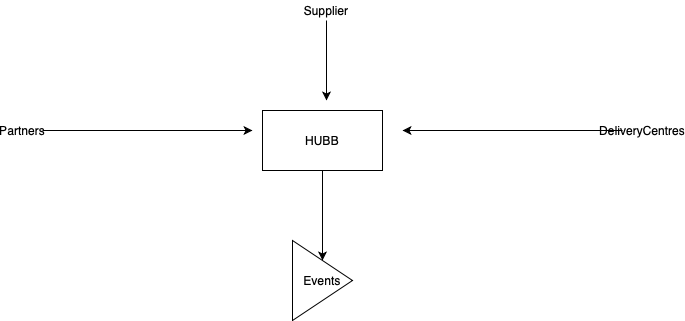
\includegraphics[scale=0.5]{hubb}

\begin{lstlisting}
	createData()
	parseData()
	processData()
		identify()
		extract()
		reshape()
	return()	
\end{lstlisting}

   
\section{Eventing Layer}

An eventing layer plays a vital role in the process of COVID-19 vaccination drive. It involves sending out important alerts and notices regarding vacine availability, vaccine shipping from particular location, vaccine production updates, and related information in real-time to the interested parties and services involved in a vaccination process. The eventing layer includes pre-defined steps and processes, but in case of deviation in any of these steps, an eventing layer is supposed to send out notifications to involved parties. It includes vaccine shortage, vaccine expiry, excess vaccine availability, or changes in timelines.

Eventing layer service is used to manage end to end shipping and define event points that can be flow, or logical steps, or an incident. When an incident is triggered at any level, parties are notified that supports improved decisions on the vaccine distribution to the most needed locations. A practical example includes notices and alerts of vaccine delivery at the site and who delivered when vaccine supply reaches the tampered unit.

This eventing layer can use the above data layer to identify parameters from data attributes, like when and whom to send notifications. Such type of eventing layer already exists in modern web apps nowadays, specifically in machine learning.    

\section{AI}
AI is a powerful technology with human-like intelligence that works as a catalyst in enhancing performance and efficiency of systems. The application of AI in the healthcare sector is notably visible such as drug discovery. Scientists are rapidly implementing inexpensive AI-enabled technologies to find therapies. AI should support the fair, transparent, just, accountable use in these technologies as meeting the challenge of demand forecasting and supply chain management is acute in controlling the COVID-19 pandemic. If given enough date, the machine can aid the search of the drug\cite{keshavarzi2020artificial}. IBM has used satellite imagery and maps, official government data, social media posts, and a number of mobile phone users in a certain area in African projects to predict the number of people that will show up at the healthcare centre. IBM system combines several datasets to analyse and make accurate predictions \footnote{https://fortune.com/2021/01/06/covid-vaccine-rollout-distribution-vaccination-coronavirus-ai-blockchain/}.  

Once we build the information that allows us to have quality data with few errors, we can use sophisticated math models and train machines using reinforcement learning. Hence, trained machines can help in predictions for forecasting inventory, preparing for hazards, analysing the turnaround time based on the optimal functioning of the overall supply chain. We describe these models here that can be fed in any application to achieve optimal distribution.

\begin{enumerate}
	\item Present vaccine distribution largely focuses on the individual at risk. We can use spatiotemporal regions for the newest cases of infection during a certain time frame and compare them with the standard practice of demographical vaccines distribution. A computational model presented in\cite{grauer2020strategic}, for a locally well-mixed population, strongly reduces the number of deaths by 35\%. The model emphasises the density of the population in a given space and time ie a region, targets using a math-based model and realises herd immunity.
	\item Typically, vaccines are distributed via a four-tier hierarchical network, the classic WHO-EPI model inherently is limited to meeting the demand and fixing the location of the clinic. Mixed-integer programming solves key issues of selecting storage sizes and ensures all delivery is made in a single trip\cite{yang2020optimizing}. This model is based on the following hubs and nodes associated with parental hubs. The below table shows the numerical output using the MIP model.
  
	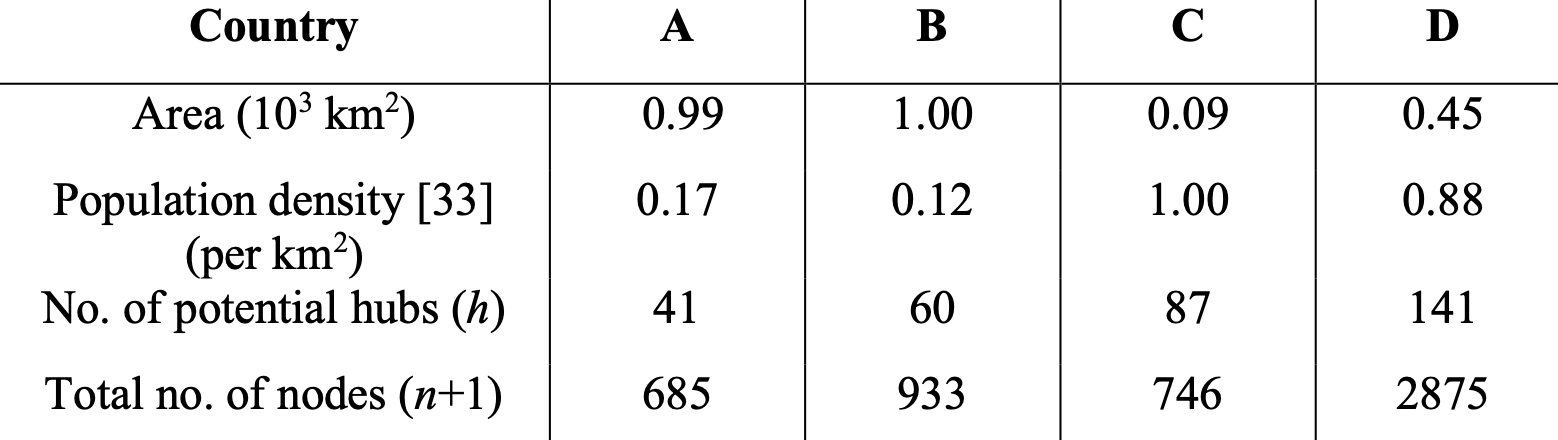
\includegraphics[scale=0.4]{maths.png}
	\item The real-world experimentation of vaccine distribution is not possible as unknown problems can occur such as scarcity of vaccine or sub-components. With enough data supplied including contextual policies with demographics for fair distribution, the resulting dynamics may change over time. The VacSim model emphasises challenges that need to be solved in real-time, without ground truth availability. This model employs the classic reinforcement learning with the forward feed that can be optimised in real-time.\cite{awasthi2020vacsim}

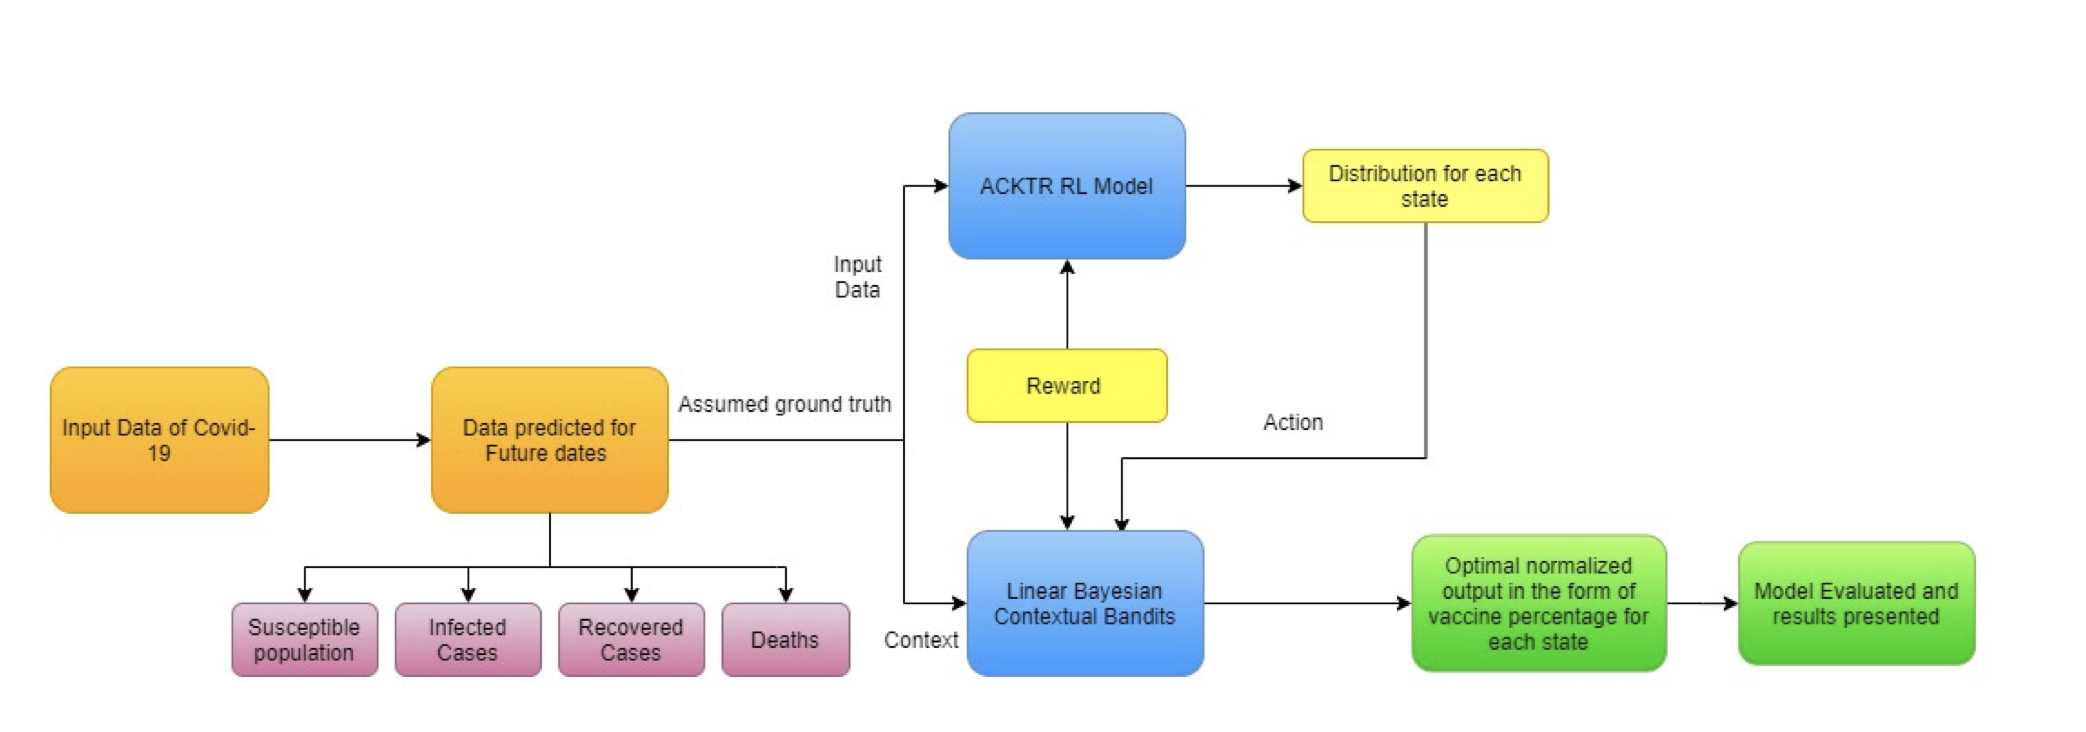
\includegraphics[width=\textwidth]{model.png}
	\item 

\end{enumerate} 

From vaccine researching, experimenting, human trial tests, and approvals to the successful vaccine delivery, it is important to ensure quality checks, streamlined production planning, warehouse management, and reduced forecast errors. ML-enabled auotmated analysis helps checking damages in vaccine production and vaacines. Ml helps in optimising the vaccine production plans using available production data and trained alogorithms. Moreover, warehouse management efficiency enhances with ML models, techniques, and forecasting features. As the COVID-19 vaccination drive is conducted all around the world at a time, it creates a large amount of dataset. ML-enabled systems are caapable of collecting, storing, processing, handling, analysing, and predicting such huge datasets while delivering near accurate insights footnote\{https://www.latentview.com/blog/how-machine-learning-can-improve-covid19-vaccine/}. Thus, AI and ML should be one of the fundamental building blocks of the vaccine distribution and supply chain network technologies and systems.

\section{Cold chain consideration}

Cold chain is the storage method of the vaccine in a provided minimum temperature range. The vaccine is a biological product that becomes ineffective over a period of time as well as when exposed to a temperature higher/ lower than the threshold or in the open air, may lose its potency. There are various other reasons for vaccine waste, like in Delhi fewer people showing up than expected\footnote{https://www.hindustantimes.com/india-news/hesitancy-causes-wastage-of-1-000-vaccine-doses-in-delhi-say-health-officials-101611091051711.html} or the delivery site having only limited storage modes that do not last for long.

\subsection{Studies}

14 and 35\% of refrigerators or transport shipments were found to have exposed vaccines to freezing temperatures, while in studies examining all the distribution segments found between 75 and 100\% of the vaccine shipments were exposed.\cite{kartoglu2014tools}. Freezing occurs when vaccine in transit uses ice packs for storage, another alternative is to use cold water packs. When developers and manufacturers design equipment to store vaccines at locations throughout the supply chain and during transport, there might be a tendency to focus on the individual user rather than the entire supply chain. But, the storage equipment sits within a larger ecosystem and characteristics such as power requirements, internal capacity, and price can have reverberating effects throughout the supply chain. Vaccine supply chain performance and efficiency depend on the ability of the system to meet storage device needs (such as maintenance technicians and spare parts) in the field. For example, the value of a passive vaccine storage device, i.e. ones that do not require a power source, depends on how well the ice supply chain can be coordinated, device mobility, and how empty devices are swapped with refilled devices.\cite{lee2017importance}
 
Currently available vaccines possess shortcomings, such as the inefficient triggering of a cell-mediated immune response and the lack of protective mucosal immunity. In this regard, recent work has been focused on vaccine delivery systems, as an alternative to injectable vaccines, to increase antigen stability and improve overall immunogenicity. In particular, novel strategies based on edible or intradermal vaccine formulations have been demonstrated to trigger both a systemic and mucosal immune response. These novel vaccination delivery systems offer several advantages over injectable preparations, including self-administration, reduced cost, stability, and elimination of a cold chain \cite{criscuolo2019alternative}

Moreover, it is essential to follow WHO guidelines for vaccine storage and distribution. According to WHO, the vaccine should be stored at 2-8\degree C [5] at every level of storage as the vaccine crosses different regions. The biological characteristic of the vaccine is impacted if it is exposed to a higher temperature than recommended. Such a vaccine may not be effective for disease prevention, ultimately increasing the demand for dosage and vaccine production. It is challenging in India to maintain and increase the capacity of a stable temperature i.e. cold chain for the existing vaccination program. Hence, coordinated efforts between regional levels are required to achieve a stable cold chain with an alternative approach that can offset the vaccine waste. 
 
 \subsection{Alternative Transformation}
 Nigeria was suffering from the lowest vaccination rates in the world due to the end-to-end approach. The nation used a strategy combining innovations in how data was captured, recorded and used to drive decision making and perform higher levels of uptime.\cite{sarley2017transforming}
 
 Methods like the HERMES computational simulation model for on-ground implementation like in the case of Mozambique resulted in 27\% vaccine delivery. The alternative system also produced higher availability at lower costs after new vaccine introductions.\cite{LEE20164998}
 
 In some situations, it is more efficient to bring the vaccines to the people instead of the other way around. Mobile medical teams need to route vaccines from one location to another. Halper and Raghavan define the mobile facility routing problem, with moving facilities to serve demand at different nodes in the network. In the case of multiple facilities, the routing problem is NP-hard and a heuristic is proposed to solve the problem.\cite{duijzer2018literature}
 
 To improve instant action and fallback strategies like what to do when a temperature falls below a certain level, constant data loggers as described above in the eventing layer section and data layer for synchronised behaviour across all domains are used.
 
 \subsection{Handling Waste}
 
One of the major environmental problems noticed with COVID-19 pandemic started was the medical waste generated in the treatment such as protective clothes and quipment  such as masks, gloves, aprons, and bottles of sanitizers. The management of infectious medical waste during COVID-19 pandemic was a big challenge for waste management departments. Since the pandemic started, the world produced about 1.6 million tonnes of medical plastic waste every day. It included around 3.4 billion single use face masks/ face shields discarded daily \footnote{https://www.sciencedirect.com/science/article/pii/S2405844021004485}. 

Design of the medical waste supply chain is critical for supplies that have been used for infectious patients, where the risk of further transmission is always imminent. A sustainable, pollution-free, and emission-free waste management systems and methods need to be implemented to process all the medical waste generated and to reduce the landfills. Pishvaee et al. (2014) proposed a method to design a sustainable medical supply chain, considering the complete life cycle of medical supplies and waste. Saif and Elhedhli (2016) took environmental considerations into account when studying the design of a cold supply chain. \cite{duijzer2018literature} The integration of environmental and social considerations should be incorporated while designing a waste management system.
 
 \subsection{Integration}
 The WHO recommends integrating the vaccine supply chain with other health supply chains. Yadav et al. (2014) studied the possibilities of such integration. According to their opinion, though outsourcing can be beneficial, it is important to consult all stakeholders in advance. The study provides illustrations of successful integration from which lessons can be learnt. The authors conclude that it is highly important to carefully determine which parts of the supply chain should be outsourced and to whom.\cite{duijzer2018literature}
 
 In India, there are various methods like using public and private transport infrastructure for delivery methods. Private companies like Uber and Ola have built technology to map faster routes with maximum optimisation of end to end delivery. One use case is utilising the existing fleet to transport vaccines internally in a local region.
\section{Cryptographic Methods}

Data privacy is one of the key parameters to be sure of while delivering vaccines throughout the network A process defines how data is governed internally and how it is going to be shared with stakeholders. This data includes health records and constant monitoring of the users, therefore data security is an important pillar in the vaccine network. Government systems are highly centralised in nature that trade-off the security requirements. 
	
\section{Challenges}

One of the most distressing fact about COVID-19 vaccination delays is the unwillingness of people to get vaccinated. Recent studies indicate 71\% of individuals from 19 countries would take vaccines. Whereas, countries like Russia have only 55\% of people that are willing to participate in the exercise. MOreover, misinformation spread through social media campaigns or personal accounts presents additonal threat to the efforts in controlling the pandemic. Though the magnitude of the pandemic has reduced in some parts of the world and are under control in others, it is essential to get vaccinated for all people. 

Governments will have a tough time ahead convincing people to get vaccinated. Today, governments need to fundamentally gain trust and understanfing along with shifting their view. Health campsings should deliver quality and right information and directly motivate citizens with the use of effective data-driven planning and dialogue. Presently, countries like India have scientists from all across different domains who are raising voices against vaccine production and its efficacy since some vaccines did not even go to phase 3. Though vaccine hesitancy and misinformation challenges are not new, these issues are serious and can be addressed with transparent processes, high regulateoty standards and works to strengthen vaccine production, supply chain and distribution systems.

\subsection{Transparency}

People in the 21st century demand all the details of the products they are buying, consuming and using, and vaccines are not an exception. Though most people are not having the background, they want simplified explanations for vaccine production, deliveries, care to be taken prior and post vaccination, and so on. Being transparent to provide all the basic information regarding available vaccine data, their benefits, side-effects, distribution and research & development is the fundamental right of people that are going to be vaccinated. Vaccine builders and governments have to be open and clear about the data that it provides to users. It will not only build trust and understanding between vaccine providers and people but also will increase people's involvement in the global COVID-19 vaccination campaign.

\subsection{Building for Future}

Existing systems lack synchronicity, connectivity, reliability, transparency, and usability in the entire vaccine distribution and supply chain network and events. Though their are few systems developed to tackle most present issues, technology is also evolving rapidly that needs systems to integrate with updated and upgraded technologies. In case of vaccine distribution and supply chain network, the government needs to start building platforms and systems with the future approach. Technology can be used where value driven systems are in place and citizens can access true information from the government about their health.	

All systems in the network should be connected and available 24*7. It will enable decision makers, manufacturers, and distributors to determine vaacine requirements and accordingly developing cold storage systems. Additionally, the security of the private as well as health data provided in the vaccination drive should be safe and secure in all extreme natural events and cyber threats. To mitigate these issues, the data privacy and security technology should be developed, maintained, and updated time to time.  
  
\section{Conclusion}
The COVID-19 pandemic disrupted the world within weeks and lockdown situation lasted for more than a year. The record breaking number of infections and deaths forced scientists to develop vaccine to reduce the severe impacts of the COVID-19 virus. Numerous vaccines were permitted to vaccinate people without following all the rules and regulations strictly to control the pandemic. Though it definitely reduced severity of infections to some extent, the effective vaccine distribution and supply chain network could have helped in controlling the spread of a disease significantly. Each country has its own challenges to deal while supplying vaccines sufficiently to its people such as vaccine unavailability or shortage, cold chain inefficiency, synchronicity, updated solutions, communication channels and integration of different eventing layers. The paper discussed these challenges in detail and suggested solutions to make COVID-19 vaccine distribution and supply chain netowrk effecient, effective, reliable, and secure. The transparency is one of the crucial parameter for governments and vaccine suppliers to gain people's trust and boost the involvement of people in the gloabl vaccination drive.    

\bibliographystyle{aabbrv}
\bibliography{bib/graph}


\end{document}




